\documentclass[withoutpreface,bwprint]{cumcmthesis}
%这里是导言区
\usepackage{url}
\usepackage{epsfig}
\usepackage{graphicx}
\usepackage{amsmath}
\usepackage{diagbox}
\usepackage{algorithm}
\usepackage{listings}
\usepackage{algpseudocode}
\usepackage{appendix}

\title{数值代数十一上机作业}
\date{\today}
\author{Jinze Wu 1700010643}
\begin{document}
\maketitle
\section{上机作业1}
\subsection{问题描述}
对单位正方形上的possion方程:

\begin{equation}
\left\{
\begin{array}    {lr}    
   -\triangle u =f & in    \Omega  \\     
        u=0        & \partial \Omega        
      \end{array}
\right.
\end{equation}
其中$f=2\pi^{2}sin(\pi x)sin(\pi y)$, $\Omega=[0,1]\times[0,1]$,真解为$u=sin(\pi x)sin(\pi y)$

利用五点差分法求解:

离散化:
\begin{align}
x_i=ih,i=0,1,\dots,N &\\
y_j=jh,j=0,1,\dots,N
\end{align}
其中N=1/h

对内部节点
\begin{equation}
\frac{2u_{i,j}-u_{i+1,j}-u_{i-1,j}}{h^{2}}+\frac{2u_{i,j}-u_{i,j+1}-u_{i,j-1}}{h^{2}}=f(x_{i},y_{j})
\end{equation}
其中$i=1,\dots,N\quad j=1,\dots,N$

对边界节点,代入边界条件
\begin{alignat}{2}
u_{i,j} & = 0 & \qquad on\partial \Omega 
\end{alignat}

得到一个$(N-1)\times(N-1)$阶线性方程组:
\begin{equation}
\begin{bmatrix}
\frac{A_{N-1}}{h^2} & -\frac{I_{N-1}}{h^2}&       &       \\
\frac{-I_{N-1}}{h^2} & \frac{A_{N-1}}{h^2}&\frac{-I_{N-1}}{h^2}&        \\
        & \ddots &\ddots &\ddots \\
        &        &\frac{-I_{N-1}}{h^2}&\frac{-A_{N-1}}{h^2} \\
\end{bmatrix}
\begin{bmatrix}
U_1\\
U_2\\
\vdots\\
U_{N-1}
\end{bmatrix}
=
\begin{bmatrix}
f_1\\
f_2\\
\vdots\\
f_{N-1}
\end{bmatrix}
\end{equation}
其中$I_{N-1}$为N-1阶单位矩阵,
\begin{equation}
A_{N-1}=
\begin{bmatrix}
4 & -1     &  &  \\
-1 & 4     &-1 &\\
  & \ddots&\ddots&\ddots\\
  &       & -1 & 4
\end{bmatrix}
\quad U_i=
\begin{bmatrix}
u_{i,1}\\
u_{i,2}\\
\vdots\\
u_{i,N-1}
\end{bmatrix}
\quad f_i=
\begin{bmatrix}
f(x_i,y_1)\\
f(x_i,y_2)\\
\vdots\\
f(x_i,y_{N-1})
\end{bmatrix}
\end{equation}
这里$i=1,2,\dots,N-1$

对$N=9,10,\dots,99$

分别用Gauss消去法,$LDL^T$方法,带状Gauss消去法,matlab现有程序包求解

以下画出运算时间随N的变化曲线

\begin{figure}[!h]
\centering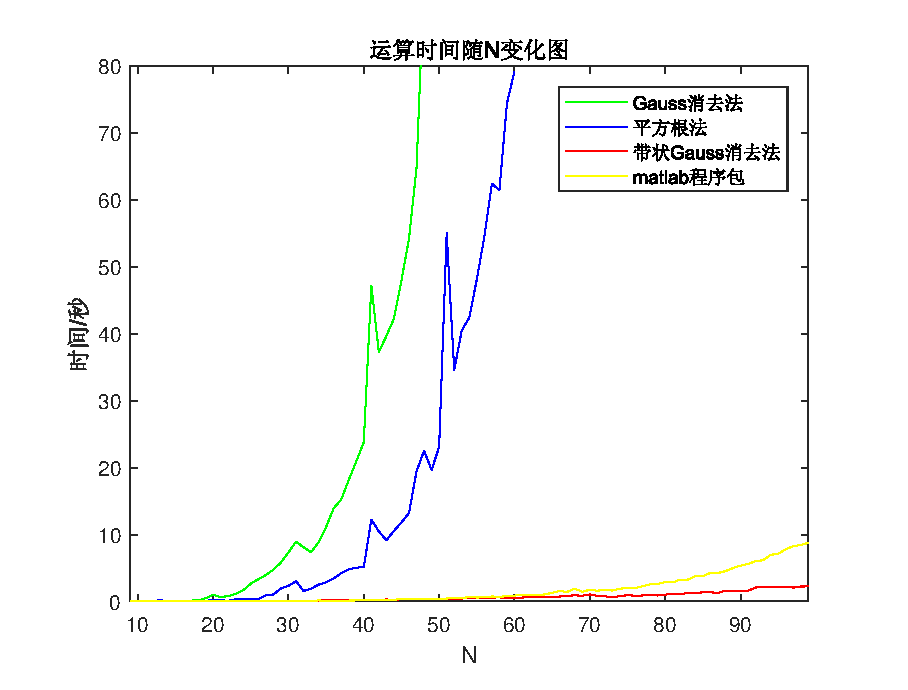
\includegraphics[width=.6\textwidth]{计算时间.eps}
\end{figure}

\begin{figure}[!h]
\centering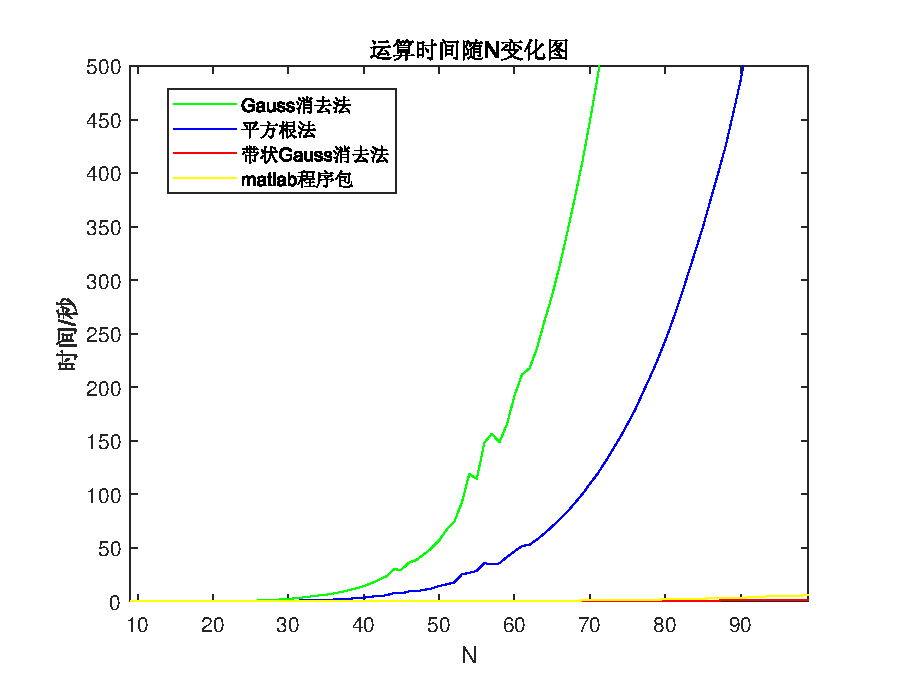
\includegraphics[width=.6\textwidth]{计算时间3.eps}
\end{figure}

总结:一般的Gauss消去法运算量约为$\frac{2}{3}N^6$,$LDL^T$方法,所需要的运算量约为$\frac{1}{3}N^6$,对大规模的矩阵算起来特别慢。
而带状Gauss消去法运算量约为$O(N^4)$,当矩阵规模增大时带状Gauss消去法相比于之前两种大大缩短了计算时间,并且比用matlab中已有的程序包求解还要快一些。

\section{上机作业2}
A为40阶Hilbert矩阵,即A的第i行第j列元素为
\begin{equation}
a_{i,j}=\frac{1}{i+j-1}
\end{equation}
向量b第i个分量为
\begin{equation}
b_i=\sum_{j=1}^n\frac{1}{i+j-1}
\end{equation}
求解线性方程组Ax=b,真解为$x=[1,1,\dots,1]^{T}$

分别用平方根法,改进平方根法,matlab现有程序包求解,用列主元Gauss消去法计算:

利用平方根法计算时间为0.002s,误差$\lVert x_{1}-x \rVert_{2}=11.4397$

用改进平方根法计算时间为0.003s,误差$\lVert x_{2}-x \rVert_{2}=11.5916$

用列主元Gauss消去法计算时间为0.006s,误差$\lVert x_{3}-x \rVert_{2}=739.9179$

用matlab程序包求解计算时间为0.001s误差$\lVert x_{4}-x \rVert_{2}=240.7459$

总结:问题中矩阵规模比较小,用各种方法求解都很快,计算时间差异不大,改进平方根法计算时间比平方根法稍快,符合预期。$n \times n$的Hilbert矩阵条件数随n指数增长$O((1+\sqrt{2})^{4n}/\sqrt{n})$,过于病态,用各种方法运算时间相差不大,且都会有较大误差,但用平方根法与改进平方根法误差相对较小。
\end{document}